\section{Auswertung}%
\label{sec:auswertung}

Ziel der Auswertung ist es einerseits, das Verhältnis der Radiumisotope
$^{85}$Rd und $^{87}$Rd zu bestimmen, sowie die Land\'efaktoren $g_\text{F}$ und
die Kernspins $I$.
Desweiteren wird das Erdmagnetfeld einerseits über eine statische
und andererseits über eine dynamische Methode bestimmt.
\subsection{Bestimmung des Erdmagnetfeldes}%
\label{sub:statische_bestimmung_des_erdmagnetfeldes}
\begin{wrapfigure}[15]{l}{0.45\textwidth}
	\centering
	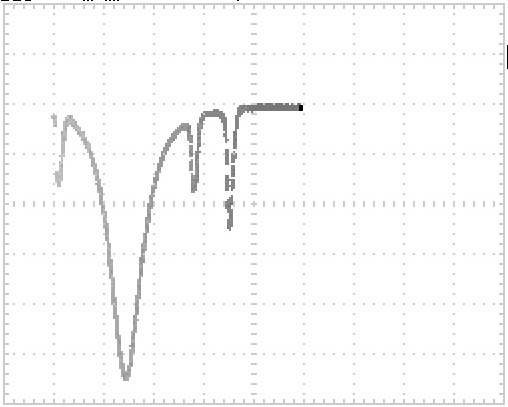
\includegraphics[width=\linewidth]{picture/Transmission_Spek_cut.JPG}
	\caption{Transmissionslinien der Rubidiumisotope $^{85}$Rb und $^{87}$Rb bei
	einer Anregungsfrequenz von \SI{100}{\kilo\hertz}.}%
	\label{fig:transmission}
\end{wrapfigure}
Das Magnetfeld der Helmholtzspulen wird anhand von Formel~\ref{eq:helm}
berechnet.
Dazu wird das Magnetfeld der Sweepspule und der horizontalen Spule addiert.
Durch das Wechseln der Sweepspule vom kontinuierlichen auf den statischen Betrieb
können die Resonanzstellen im Spektrum abgefahren werden.
In Abbildung~\ref{fig:transmission} ist der Photostrom gegen die Frequenz der
RF-Spule aufgetragen.

\subsubsection{Statische Methode}%
\label{ssub:subsubsection_name}
Der große Peak entspricht grade dem Magnetfeld, welches die Horizontalkomponente
des Erdmagnetfeldes $B_\text{Erd}$ kompensiert.
Die Vertikalkomponente wird optimiert, sodass der Peak möglichst schmal ist.
Es ergibt sich ein Magnetfeld von
\begin{eqnarray}
	B_\text{Erd,horiz} =& \SI{36.7}{\micro\tesla}, \\
	B_\text{Erd,verti} =& \SI{19.3}{\micro\tesla}.
\end{eqnarray}

\subsubsection{Dynamische Methode}%
\label{ssub:dynamische_methode}
Zur Bestimmung des Erdmagnetfeldes über die dynamische Methode werden die
Resonanzstellen der beiden Isotope vermessen und linear gefittet.
Die angelegten magnetischen Felder $B$ sind in Abhängigkeit der Frequenz in
Tabelle~\ref{tab:b_nu} aufgeführt.
Die Magnetfelder $B$ aufgetragen gegen die Anregungsfrequenzen $\nu$ sind in
Abbildung~\ref{fig:static_B} zu sehen.
\begin{table}[h]
	\centering
	\caption{Magnetfeld zur Einstellung der Resonanz der Rubidium Isotope.}%
	\label{tab:b_nu}
	\sisetup{%
		round-mode=places,
		table-format=3.1,
		round-precision=1,
	}
		\input{build/b_nu.tex}
\end{table}
Die Messwerte werden linear gefittet und der y-Achsenabschnitt $b$
entspricht genau dem Offset, den das Erdmangnetfeld erzeugt.
\begin{figure}[h]
	\centering
	\includegraphics[width=0.8\linewidth]{build/static_B.pdf}
	\caption{Linearer Zusammenhang der Resonanzfrequenz und dem angelegten
	magnetischen Feld für beide Isotope.}%
	\label{fig:static_B}
\end{figure}
Das zur Kompensation des Erdmangnetfeldes benötigte Feld entspricht dem Wert $b$ aus
Tabelle~\ref{tab:lin_params}.
\begin{table}[h]
	\centering
	\caption{Lineare Fitparameter zur Bestimmung des Land\'efaktors und des
	Erdmagnetfeldes.}%
	\label{tab:lin_params}
	\sisetup{%
		round-mode=figures,
		round-precision=3,
		table-format=1.2e3
	}
	\input{build/lin_params.tex}
\end{table}
\subsection{Land\'efaktoren und Kernmoment der Rubidium Isotope}%
\label{sub:landefaktoren_der_rubidium_isotope}
Die Land\'efaktoren werden entsprechend Gleichung~\ref{eq:lande} aus der Steigung
des Fits in Abbildung~\ref{fig:static_B} bestimmt.
Durch Umformen ergeben sich die in der Tabelle~\ref{tab:lande} aufgeführten
Land\'efaktoren $g_\text{exp}$ und die theoretischen Werte $g_\text{theo}$.
\begin{table}[h]
	\centering
	\caption{Die abgeleiteten Größen: Land\'efaktor und Kernspin aus der Steigung
	$\nu$ gegen $B$.}%
	\label{tab:lande}
	\begin{subtable}[t]{0.4\textwidth}
	\centering
	\caption{Land\'efaktoren}%
	\label{tab:label}
	\input{build/lande.tex}
	\end{subtable}
	\begin{subtable}[t]{0.4\textwidth}
	\centering
	\caption{Kernspins}%
	\label{tab:label}
	\input{build/kernspin.tex}
	\end{subtable}
\end{table}

\begin{table}[h]
\end{table}
\subsection{Quadratischer Zeemanneffekt}%
\label{sub:quadratischer_zeemanneffekt}
Der quadratische Zeemanneffekt führt zu einer Energieabsenkung.
Er liefert erst bei größeren Feldstärken signifikante Beiträge.
Zur Abschätzung wird eine Feldstärke von $B=\SI{1}{\milli\tesla}$
und die Land\'efaktoren von Rubidium angenommen und die Energien entsprechend
Formel~\ref{eq:quad_zee} ausgerechnet.
\begin{equation}
	\frac{E_\text{squ} = \SI{1.04 +- 0.01e-29}{\joule}}{E_\text{lin} =
		\SI{4.57 +- 0.02e-27}{\joule}} \approx 0.2 \%
\end{equation}
Er kann bei kleinen Feldern von um die \SI{100}{\micro\tesla} vernachlässigt werden.

\subsection{Bestimmung des Isotopenverhältnis}%
\label{sub:bestimmung_des_isotopenverhaeltniss}
Zur Bestimmung des Isotopenverhältnis wird einerseits eine statische Methode,
welche auf dem Amplitudenverhältnis der Transmissionslinien beruht,
und andererseits eine dynamische über die Rabi-Oszillationen gemessen.
\subsubsection{Statische Methode}%
\label{ssub:statisch}
Das Amplitudenverhältnis kann aus der Abbildung~\ref{fig:transmission} abgelesen werde.
Dabei entspricht die erste Transmissionslinie dem $^{85}$Rb und die zweite dem
$^{87}$Rb Isotop.
Es wird ein Amplitudenverhältnis von
\begin{equation}
	\frac{A_{85}}{A_{87}} = \frac{\SI{2.6}{\volt}}{\SI{1.4}{\volt}} = \num{1.86}
\end{equation}
gemessen, was von dem natürlichen um \SI{39.4}{\percent} und vom angegebenen
theoretischen Wert um \SI{20}{\percent} abweicht.
Augenscheinlich wurde das Rubidiumgas mit dem $^{87}$Rb Isotope angereichert,
um bessere optische Eigenschaften zu erreichen.


\subsubsection{Dynamische Methode}%
\label{ssub:dynamisch}

Zur Bestimmung des Isotopenverhältnis werden bei einer RF-Frequenz von
\SI{100}{\kilo\hertz} die Spulenspannung variiert und die Oszillationen gemessen.
Die entsprechende Schwingungsdauern bei den verschiedenen Spannungen sind in
Tabelle~\ref{tab:schw} aufgetragen.
Ein Oszilloskopbild ist für beide Resonanzstellen in
Abbildung~\ref{fig:osz} zu sehen.
\begin{figure}[h]
	\centering
	\begin{subfigure}[c]{0.45\textwidth}
	\begin{center}
	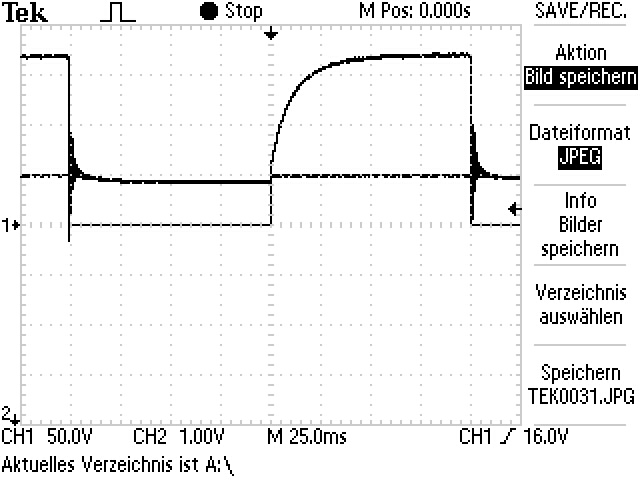
\includegraphics[width=\textwidth]{./picture/Peak_1.JPG}
	\end{center}
	\caption{$^{85}$Rb}%
	\label{fig:}
	\end{subfigure}
	\begin{subfigure}[c]{0.45\textwidth}
	\begin{center}
	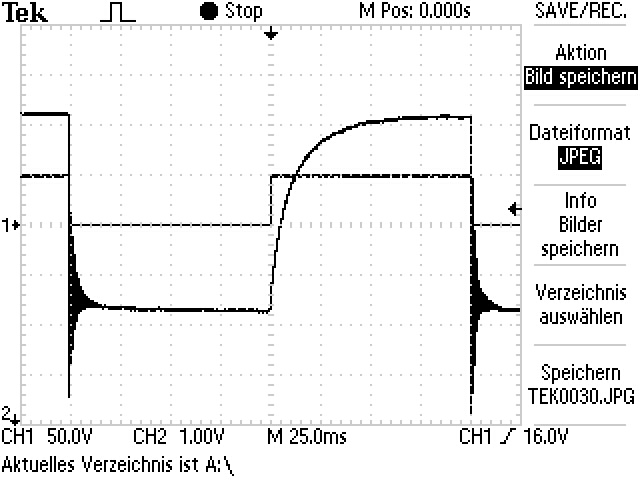
\includegraphics[width=\textwidth]{./picture/Peak_2.JPG}
	\end{center}
	\caption{$^{87}$Rb}%
	\label{fig:}
	\end{subfigure}
	\caption{Ladung und Entladung des Gases mit Anregung und anschließenden
  Oszillationen.}%
	\label{fig:osz}
\end{figure}
Die Periodendauern werden bestimmt, indem mit der
Funktion \texttt{scipy.signal.find\_peaks}
die Extrema der periodischen Funktionen bestimmt werden.
Bei kleinen Spulenspannungen kommt es dabei zu Untergrundrauschen und
Beeinflussung durch hohe Magnetfelder der nebenstehende Experimente
(Abbildung~\ref{fig:85a}), sodass die Periode nicht mehr eindeutig
bestimmt werden kann.
Desweiteren wurde die zeitliche Auflösung, zur Bestimmung der Periodendauer
der zweiten Transmissionslinien etwas zu grob gewählt, sodass die
Schrittweite zum Teil sehr groß ist.
Die bestimmten Periodendauern sind in Tabelle~\ref{tab:schw} aufgelistet.
\begin{table}[h]
	\centering
	\caption{Periodendauern der Larmorschwingungen.}%
	\label{tab:schw}
	\begin{subtable}[t]{0.4\textwidth}
	\centering
	\caption{$^{85}$Rb}
		\input{build/T1.tex}
	\end{subtable}
	\begin{subtable}[t]{0.4\textwidth}
	\centering
	\caption{$^{87}$Rb}
		\input{build/T2.tex}
	\end{subtable}
\end{table}
In der Abbildung~\ref{fig:periode} sind die Feldstärken gegen die Spulenspannungen
aufgetragen und die Messdaten mit der Funktion~\ref{eq:fit} gefittet.
\begin{figure}[h]
	\centering
	\begin{subfigure}[c]{0.45\textwidth}
	\begin{center}
		\includegraphics[width=\textwidth]{build/firstPeak_9.png}
	\end{center}
	\caption{$^{85}$Rb \SI{10}{\volt}}%
	\label{fig:}
	\end{subfigure}
	\begin{subfigure}[c]{0.45\textwidth}
	\begin{center}
		\includegraphics[width=\textwidth]{build/secondPeak_9.png}
	\end{center}
	\caption{$^{87}$Rb \SI{10}{\volt}}%
	\label{fig:}
	\end{subfigure}

	\begin{subfigure}[c]{0.45\textwidth}
	\begin{center}
		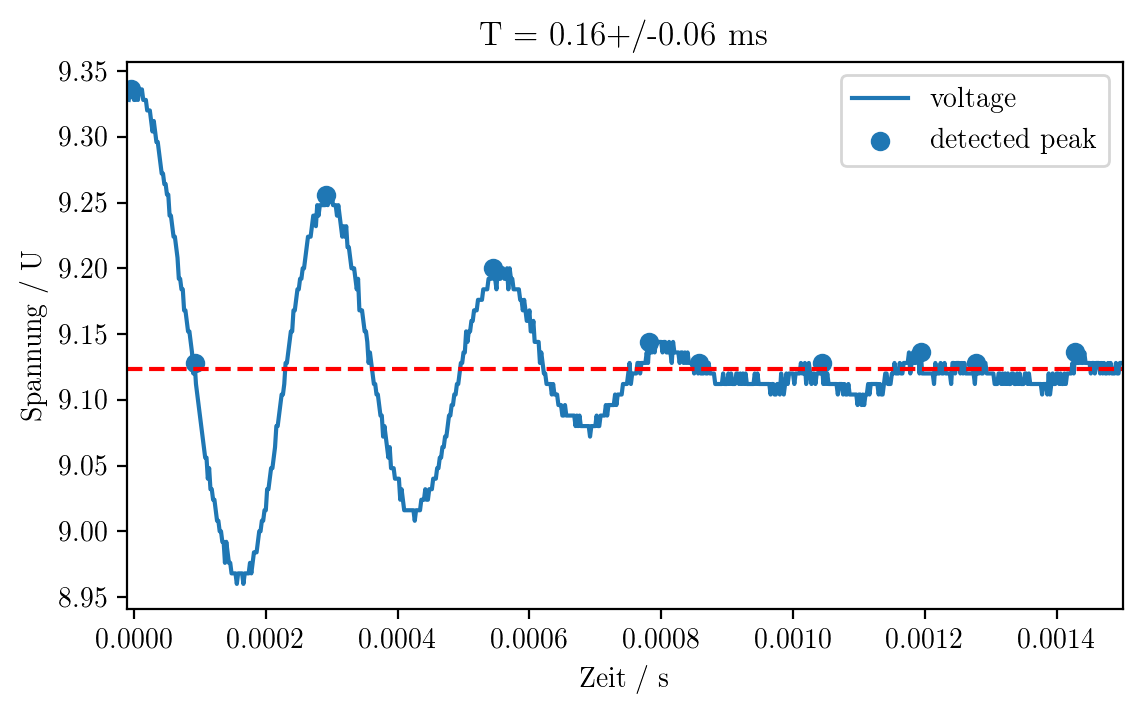
\includegraphics[width=\textwidth]{picture/firstPeak_3.png}
	\end{center}
	\caption{$^{85}$Rb \SI{1}{\volt}}%
	\label{fig:85a}
	\end{subfigure}
	\begin{subfigure}[c]{0.45\textwidth}
	\begin{center}
		\includegraphics[width=\textwidth]{build/secondPeak_3.png}
	\end{center}
	\caption{$^{87}$Rb \SI{3}{\volt}}%
	\label{fig:}
	\end{subfigure}
	\caption{Larmorschwingungen in abhängigkeit der Spulenspannung.}%
	\label{fig:periode}
\end{figure}
\begin{equation}
	\label{eq:fit}
	T(U) = a + \frac{b}{U + c}
\end{equation}
Die Ergebnisse sind in Abbildung~\ref{fig:fitexp} dargestellt.
\begin{figure}[h]
	\centering
	\begin{subfigure}[c]{0.45\textwidth}
	\begin{center}
		\includegraphics[width=\textwidth]{build/firstPeak.pdf}
	\end{center}
	\caption{$^{85}$Rb}%
	\label{fig:}
	\end{subfigure}
	\begin{subfigure}[c]{0.45\textwidth}
	\begin{center}
	\includegraphics[width=\textwidth]{build/secondPeak.pdf}
	\end{center}
	\caption{$^{87}$Rb}%
	\label{fig:}
	\end{subfigure}
	\caption{Periodendauer der Larmorschwingungen in Abhängikeit des
	Spulenspannung zur Bestimmung des Isotopenverhältnisses.}%
	\label{fig:fitexp}
\end{figure}
Aus den Verhältnissen der Steigungsparameter $b$ der Fits wird das
Isotopenverhältnis von dem Rubidiumgas abgeschätzt.
Es beträgt
\begin{equation}
	\frac{b_{85}}{b_{87}} =
	\frac{\SI{10.7+-9.0}{\second\per\volt}}{\SI{6.6+-3.5}{\second\per\volt}} =
	\num{1.6 +- 1.6}.
\end{equation}
Das natürliche Rubidium Verhältnis ist etwa 5:2.
Dies ist ein Hinweis darauf, dass das verwendete Gemisch möglicherweise für
bessere optische Eigenschaften mit dem $^{87}$Rb-Isotop angereichert ist.
Das für den Versuch angegebene Isotopenverhältnis ist 3:1.
